\documentclass[11pt]{article}
\usepackage[a4paper,margin=0.82in]{geometry}
\usepackage{fontspec}
\usepackage{xeCJK}
\usepackage{graphicx}
\usepackage{booktabs}
\usepackage{caption}

\setmainfont{Times New Roman}
\setsansfont{Arial}
\setCJKmainfont{Songti SC}
\setCJKsansfont{STHeiti}
\setlength{\parskip}{0.62em}
\setlength{\parindent}{0pt}

\title{Traditional 与 Learning-based 事件表示对比报告（最新结果）}
\author{}
\date{2026-05-20}

\begin{document}
\sloppy
\maketitle

\paragraph{Scope.} 本报告统一汇总仓库内截至 2026-05-20 的最新可用结果：N-MNIST、N-Caltech101、CIFAR10-DVS 分类结果，以及 MVSEC 统一 optical-flow protocol 结果。图表和表格均由同一脚本重新生成，旧图与旧表已清理。

\begin{figure}[t]
  \centering
  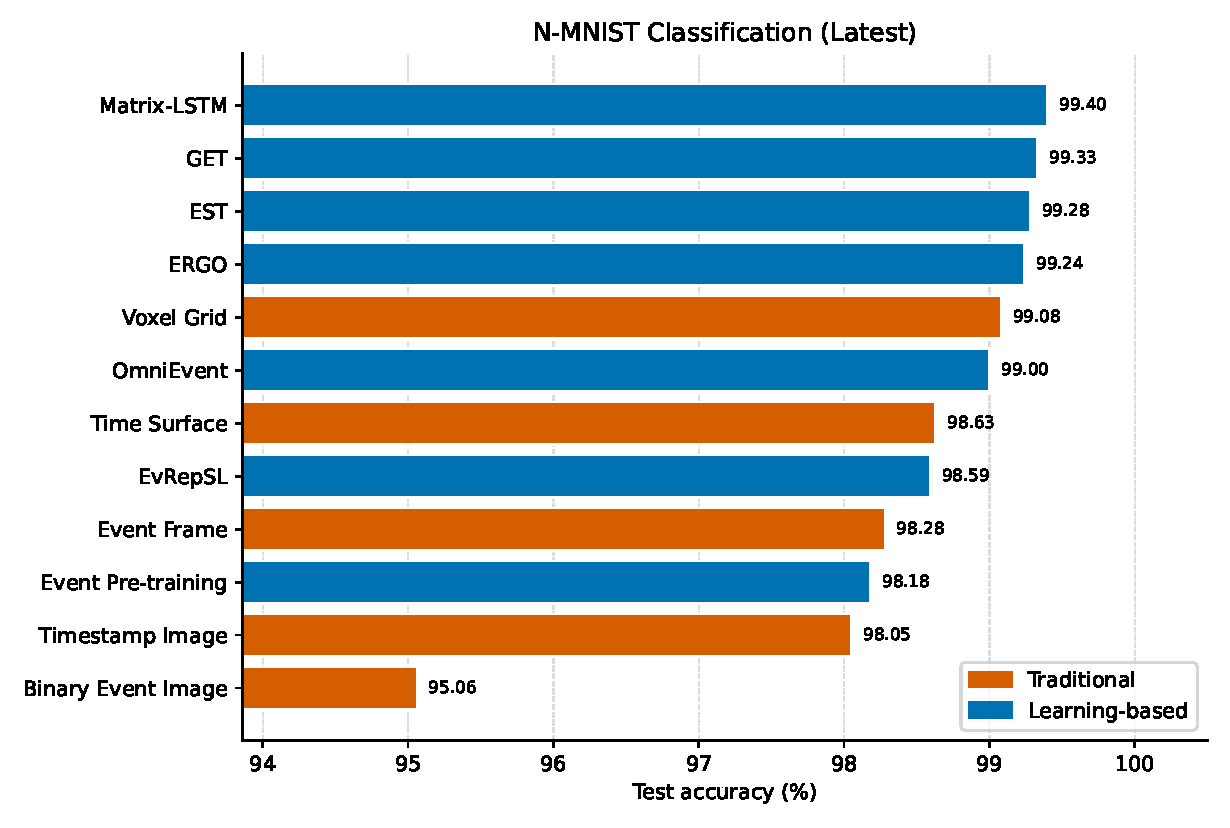
\includegraphics[width=0.90\linewidth]{nmnist_accuracy_full_aligned.pdf}
  \caption{N-MNIST 分类准确率对比（最新版）。}
\end{figure}

\paragraph{N-MNIST.} 最佳 learning-based 方法为 Matrix-LSTM (99.40\%)，最佳 traditional 方法为 Voxel Grid (99.08\%)，差距为 0.32 个百分点。该任务整体接近饱和区间。

\begin{figure}[t]
  \centering
  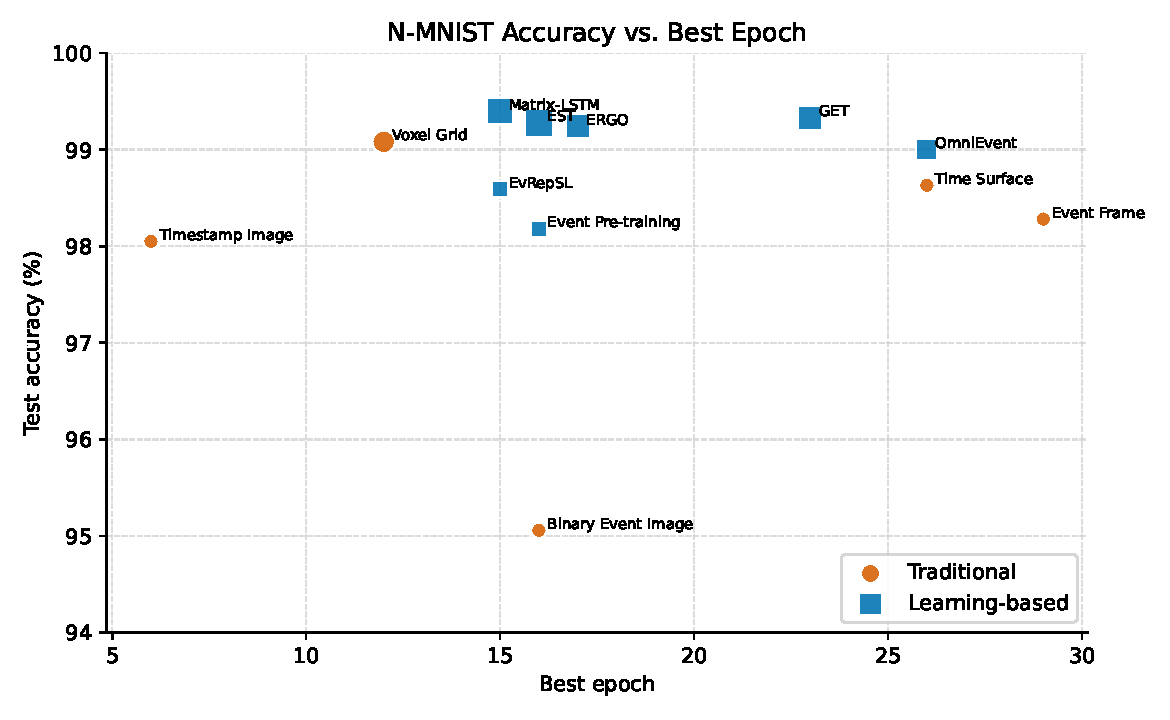
\includegraphics[width=0.88\linewidth]{nmnist_accuracy_epoch_scatter.pdf}
  \caption{N-MNIST 准确率与最佳 epoch 关系。}
\end{figure}

\begin{figure}[t]
  \centering
  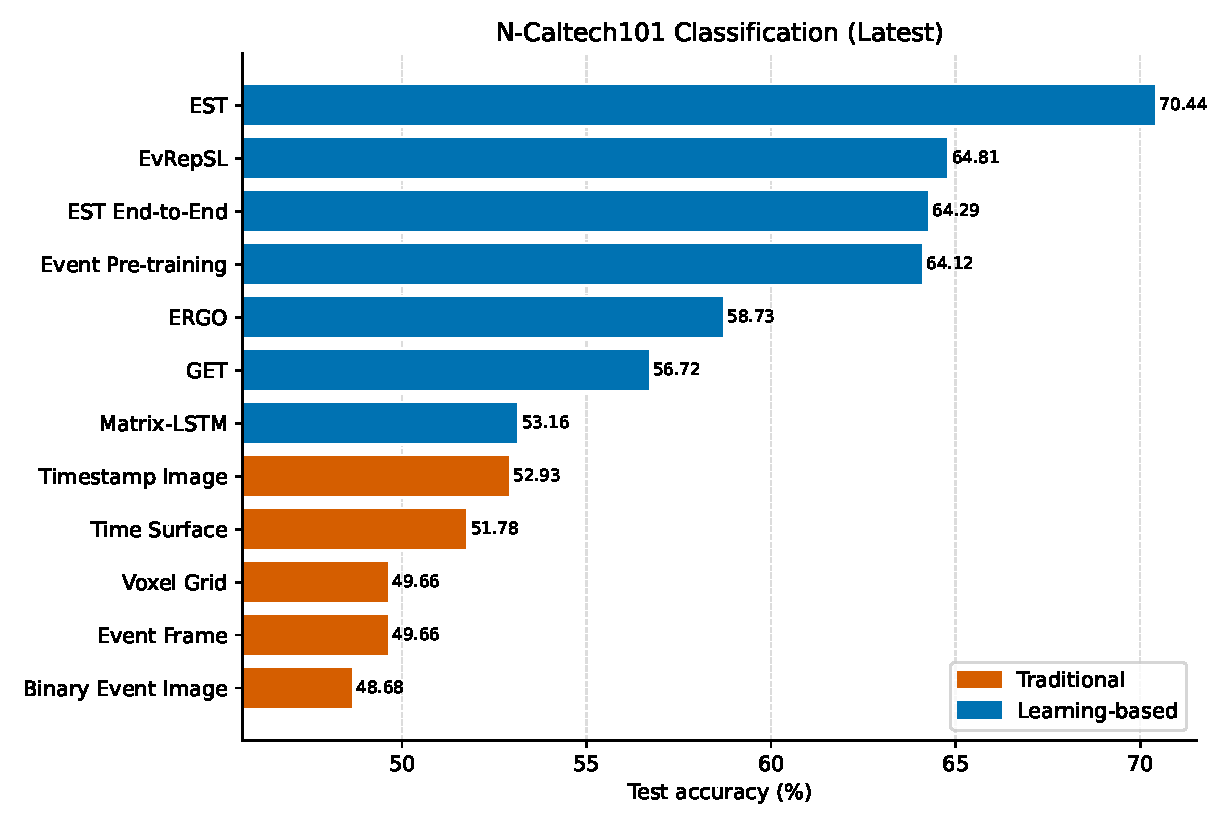
\includegraphics[width=0.92\linewidth]{ncaltech101_accuracy_full_aligned.pdf}
  \caption{N-Caltech101 分类准确率对比（最新版）。}
\end{figure}

\paragraph{N-Caltech101.} 最佳 learning-based 方法为 EST (70.44\%)，最佳 traditional 方法为 Timestamp Image (52.93\%)，差距为 17.51 个百分点。

\begin{figure}[t]
  \centering
  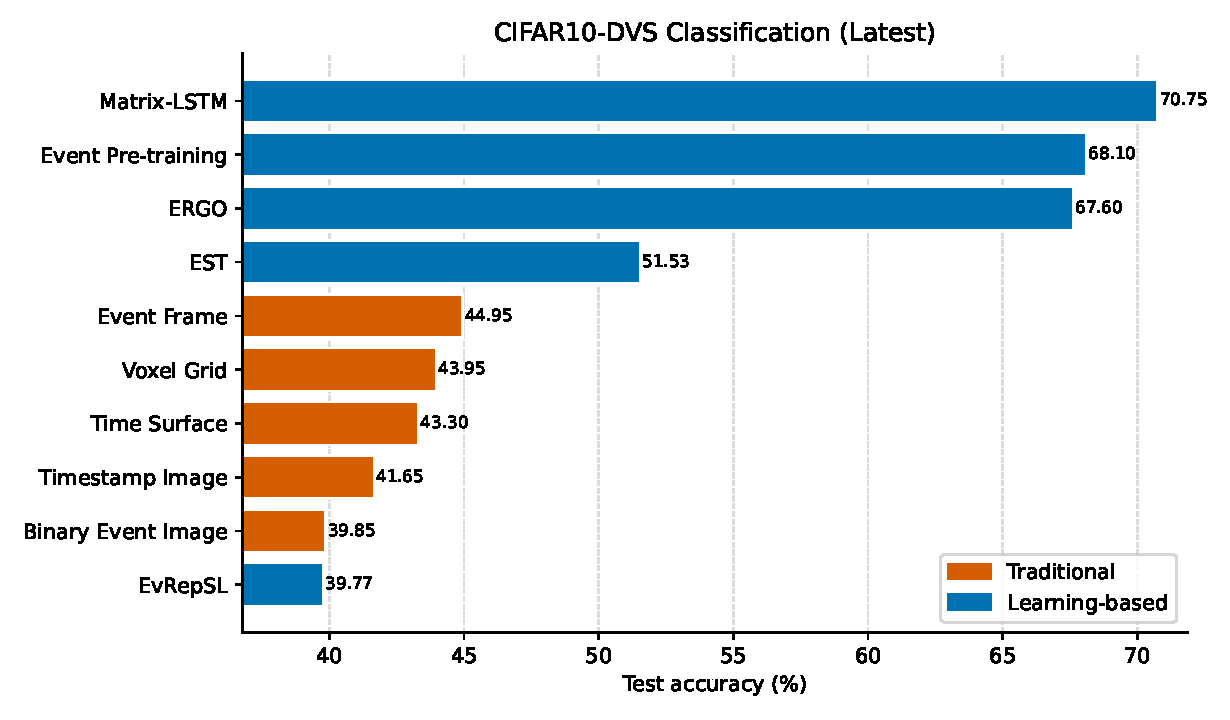
\includegraphics[width=0.92\linewidth]{cifar10dvs_accuracy_full_aligned.pdf}
  \caption{CIFAR10-DVS 分类准确率对比（最新版）。}
\end{figure}

\paragraph{CIFAR10-DVS.} 最佳 learning-based 方法为 Matrix-LSTM (70.75\%)，最佳 traditional 方法为 Event Frame (44.95\%)，差距为 25.80 个百分点。

\begin{figure}[t]
  \centering
  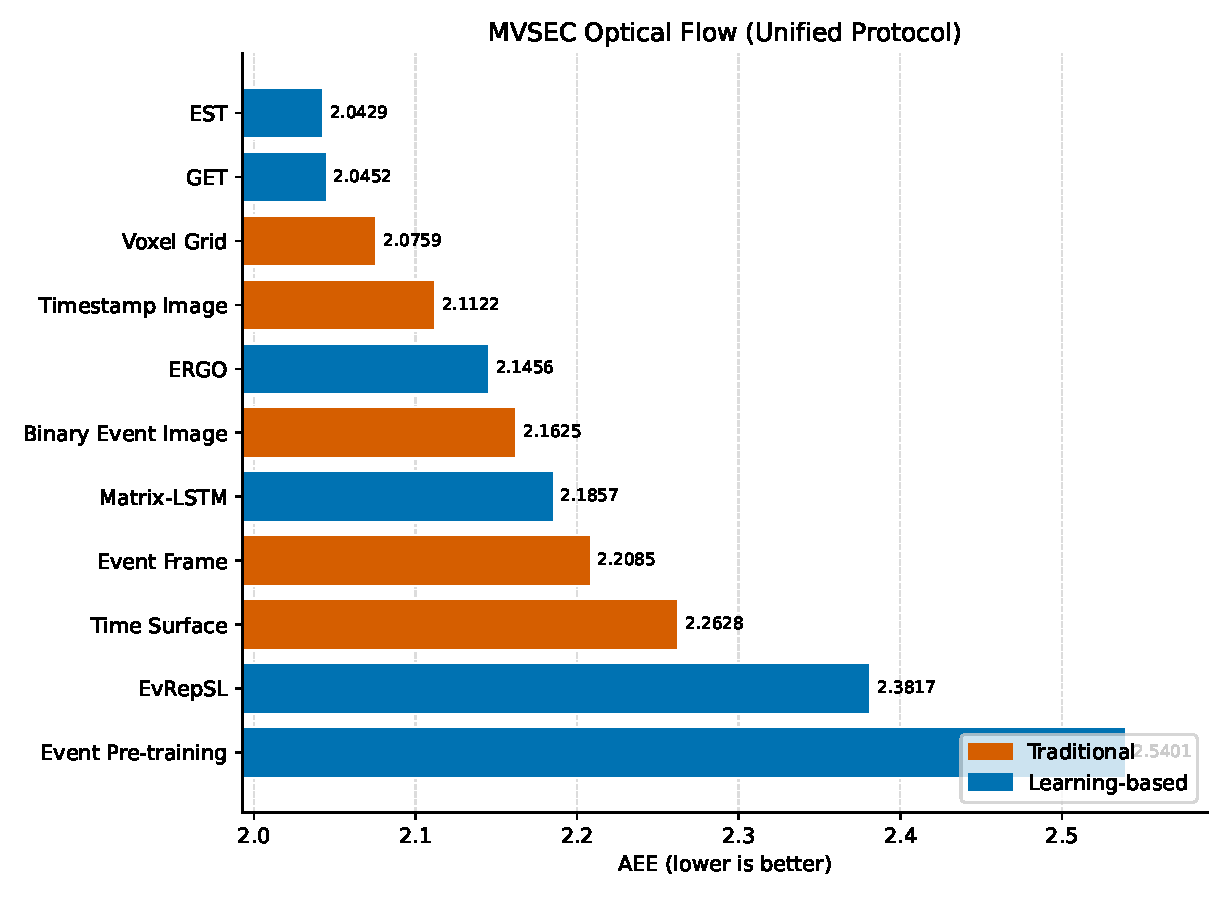
\includegraphics[width=0.88\linewidth]{mvsec_aee_full_aligned.pdf}
  \caption{MVSEC AEE 对比（统一 protocol，越低越好）。}
\end{figure}

\paragraph{MVSEC Optical Flow.} 当前总体最优为 EST，AEE=2.0429。最佳 learning-based 为 EST (AEE=2.0429)，最佳 traditional 为 Voxel Grid (AEE=2.0759)。在该统一设置下，learning 与 traditional 的最优结果差距较小。

\paragraph{Summary.} 最新结果显示：N-MNIST 上两组方法差距很小；N-Caltech101 与 CIFAR10-DVS 上 learning-based 优势更明显；MVSEC 上 traditional 仍保持竞争力。

\end{document}
